\documentclass[a4paper,11pt]{article}
\usepackage[margin=2cm]{geometry}

\usepackage[titletoc,toc,title,page]{appendix}
\usepackage[nodayofweek]{datetime}
\usepackage{cite}
\usepackage{graphicx}
\longdate



\usepackage{paralist}
\usepackage{mathcomp}
\usepackage{bm}
\usepackage{amsmath,amssymb,amsthm,enumitem}
\usepackage{graphicx}
\usepackage{caption}
\usepackage{subcaption}
\usepackage{titlesec}

\setcounter{secnumdepth}{4}

\usepackage{hyperref}
\usepackage{fancyhdr}
\usepackage{minted}
\pagestyle{fancyplain}
\fancyhf{}
\lhead{\fancyplain{}{MSc Individual Project Report}}
\rhead{\fancyplain{}{\today}}
\cfoot{\fancyplain{}{\thepage}}

\title{Information Theory and Metastability in Neural Populations\\\Large{--- Progress Report ---}}
\author{Juan Carlos Farah\\
       jcf214@doc.ic.ac.uk\\ \\
       \small{Supervisors: Professor Murray Shanahan, Pedro Mediano}\\
       \small{Imperial College London}
}

\begin{document}
\maketitle

\section{Introduction}

In the brain, metastability is defined as the ``simultaneous realisation of two competing tendencies: the tendency of the individual components to couple together and the tendency for the components to express their independent behaviour'' \cite{Kelso2012}. The Theory of Coordination Dynamics postulates that metastability is a key aspect of neurodynamics and it has been suggested that it plays an important role in several cognitive functions and consciousness \cite{Seth2009}. 

Over the past ten years, the Integrated Information Theory of Consciousness (IIT) has arisen as a possible framework to explain the nature and properties of consciousness. The IIT claims that consciousness can be measured by a system's ability to integrate information, that is, to what extent information is generated by a system as a whole and not by the sum of its parts \cite{Tononi2008a}.

By modelling synchronisation using spiking neural networks and large-scale approximations such as oscillators following the Kuramoto model, this project aims to investigate the properties of metastability and consciousness from an information-theoretic point of view. Specifically, we will conduct a series of simulations to study the correspondence between several properties of these networks, some of which are highlighted in Section \ref{Measures}, with a particular focus on how they relate to integrated information. Our goal is to shed light on the dynamics and properties of information transmission and processing between populations of neurons as they oscillate in and out of transient coupled states.

\section{Background}

This project will focus on a number of concepts from the fields of Information Theory and Computational Neurodynamics. In order to motivate their inclusion in this study and introduce the structures and measures used, this section provides a general explanation of these terms.

\subsection{Kuramoto Model}
\label{KuramotoModel}

The Kuramoto model, proposed by Yoshiki Kuramoto, is a mathematical model for a system of coupled phase oscillators. It has widespread use in neuroscience as a framework for the study of synchronisation in dynamical systems as observed in nature \cite{Cumin2007}. The dynamics of this model are an extension of work by Winfree, which Kuramoto generalised to the form below \cite{Strogatz2000}, where $N$ is the number of coupled phase oscillators $\theta_{i}(t)$ with natural frequencies $\omega_{i}$ distributed over $g(\omega)$.

$$\dot{\theta_i} = \omega_i + \sum_{j=1}^{N} K_{ij} \sin(\theta_j - \theta_i), i = 1, ..., N$$



\subsection{Networks of Spiking Neurons}

As further explained in Section \ref{MSUSNN}, we will model populations of spiking neurons in order to analyse more fine-grained properties of the network, such as its spectral complexity. The models that we will used will be based on work by Buehlmann and Deco \cite{Buehlmann2010} as well as by Bhowmik and Shanahan \cite{Bhowmik2013}. For the neurons in our networks we will use the widely used Hodgkin-Huxley model \cite{Hodgkin1952}. ``Hodgkin and Huxley found three different types of ion current: sodium (Na+), potassium (K+), and a leak current that consists mainly of chloride (Cl2) ions. Different voltage-dependent ion channels control the flow of ions through the cell membrane.'' \cite{Bhowmik2013}

For the dynamics of the neurons in our network we will follow the Quadratic Integrate-and-Fire (QIF) model. The change in membrane potential over time of QIF neurons is given by the following equations, where $V$ is the membrane potential, $V_r$ is the resting potential, $V_t$ is the firing threshold, $C$ is the membrane capacitance, $\tau$ is the membrane time  constant, $I$ is the current and $R$ the resistance.

$$ \frac{dV}{dt} = \frac{1}{\tau}(V - V_ r)(V-V_t) +  \frac{I}{C}$$
$$ \tau = RC$$

Intially, as in \cite{Bhowmik2013} we will set $\frac{1}{\tau} = 2$ and assume a membrane potential between $V_r = 265$ mV and $V_t = 245$ mV. However, depending on the results of our simulations, we might be inclined to fine-tune these values to better fit our requirements.

\subsection{Metastability}

It has been observed that ``periodic phenomena involving the synchronisation of multiple variables are prevalent both in nature and the human environment'' \cite{Shanahan2010} and these have been successfully modelled using systems of coupled oscillators such as those described in Section \ref{KuramotoModel}. Several studies have focused on investigating how these systems exhibit stable states of synchronisation \cite{Acebron2005}. However, increased long-distance synchronisation has also been linked to pathological behaviours such as epileptic seizures \cite{Arthuis2009}, which motivates the study of recurring, shorter bursts of synchronisation between oscillating structures that occur alongside periods of desynchronisation. This behaviour is defined as metastability. ``A system of oscillators exhibits metastability if some or all of its members linger in the vicinity of a synchronised state without falling into such a state permanently.'' \cite{Shanahan2010}


``Metastability is quantified by the variance of synchrony within an individual oscillator cluster over time, averaged for all clusters in the system, and so characterizes the tendency of a system to continuously migrate between a variety of synchronous states.'' \cite{Bhowmik2013}


\subsection{Chimera States}

As explained in \cite{Shanahan2010}, competition is a feature of many complex systems. In the brain, one of the ways in which competition manifests itself is in the presence of chimera states. Chimera states refer to the phenomena where a coalition of populations of neurons (or oscillators) are synchronised while other coalitions are desynchronised. This can be seen from milliseconds 310 to 330 in Figure \ref{Shanahan2010_Chimera}. We observe that the black, red, blue, green and purple communities are synchronised while the gray, turquoise and mustard communities are desynchronised.

\begin{figure}[H]
\centering
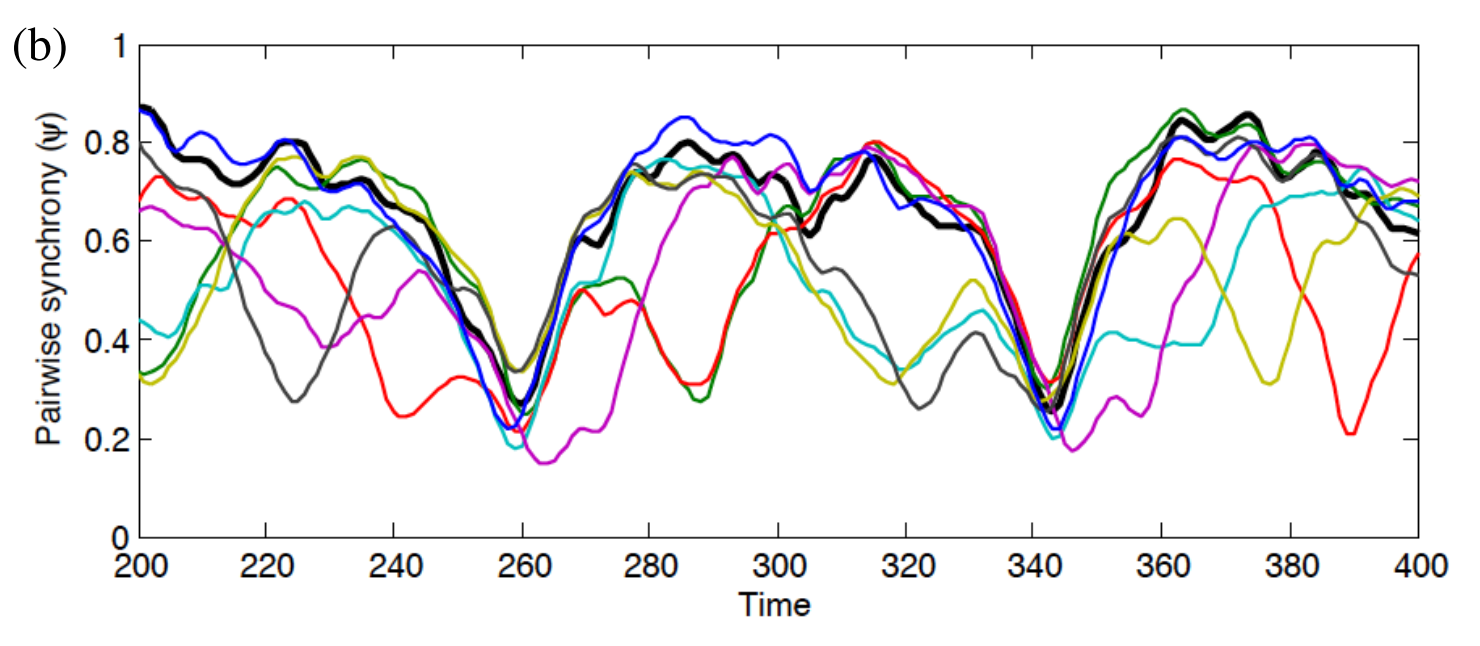
\includegraphics[scale = 0.5]{Shanahan2010_Chimera}
\caption{``Inter-community synchrony: Pairwise synchrony is plotted between one selected community (shown in black) and each of the eight communities (including itself). From time 310 to 330 the selected community is synchronised with several others, forming a temporary coalition.'' \cite{Shanahan2010}}
\label{Shanahan2010_Chimera}
\end{figure}

In order to calculate how chimera-like a system is at a given time step, we follow \cite{Shanahan2010, Bhowmik2013}, fix time and calculate the variance across communities. This indicates ``the level of spontaneous partitioning into synchronized and desynchronized subsets'' \cite{Bhowmik2013} and can be averaged as in \cite{Shanahan2010} to calculate $\chi$ shown below, where $C$ is the set of $M$ number of communities and $\psi_c(t)$ is the synchrony of community $c$ at time $t$ as described in Section \ref{Synchrony}.

$$\chi = \langle \sigma_{chi} \rangle_T$$
$$\sigma_{chi}(t) = \frac{1}{M - 1}\sum_{c \in C}(\psi_c(t) - \langle \psi(t) \rangle_C)^2$$ 


\subsection{Integrated Information Theory of Consciousness}
In 2004, Tononi presented his Integrated Information Theory, postulating that consciousness could be defined as the capacity of a system to integrate information \cite{Tononi2004}. He claimed that there were two major problems posed by consciousness. The first concerns the issue of how to determine if and to what extent a system experiences consciousness. That is, what can be measured to determine the consciousness of a given system. The second is related to the type of consciousness that a system may have. That is, addressing the fact that different kinds of conscious experiences are associated to different parts of the brain and how damage to one of these areas can affect one type of sensory experience, but leave others unaffected (e.g. certain lesions only affect one's capability to perceive colours).

We will focus on the former of these concerns. Tononi proposed that a good measure for consciousness would be $\Phi$, which computes a system's ability to generate information as a whole, rather than as a sum of its parts. We further explain integrated information in Section \ref{II}.

\subsection{Measures}
\label{Measures}
In this section we provide an overview of the different information-theoretic measure that we will use to analyse the neural populations and networks of oscillators used in this study.

\subsubsection{Entropy}

Entropy $H$ is a measure of uncertainty and for a discrete random variable $X$ that takes values in the space $\Omega_X$, can be calculated as shown below.

$$H(X) = - \sum_{x \in \Omega_X}P_X(x) \log_2 P_X(x)$$

The expected conditional entropy of $X$ given $Y$, where $Y$ is a discrete random variable that takes values in the space $\Omega_Y$, is denoted $H(X|Y)$ and calculated as shown below.

$$H(X|Y) = \sum_{y \in \Omega_Y}H(X|Y=y)P_Y(y)$$

\subsubsection{Mutual Information}

The mutual information $I(X,Y)$ between $X$ and $Y$ is the reduction in entropy of $X$ given that we know $Y$.

$$I(X,Y) = H(X) - H(X|Y)$$


\subsubsection{Synchrony}
\label{Synchrony}

The synchrony of a given community $c$ at time $t$, $\psi_c(t)$, is given by the equation below. By averaging synchrony over all communities and time steps, you can calculate global synchrony, $\Psi$ \cite{Shanahan2010}.
$$\psi_c(t) = |\langle e^{i\theta_k(t)}\rangle_{k \in c}|$$

\subsubsection{Coalition Entropy}

``Coalition entropy measures the variety of metastable states entered by a system of oscillators and is calculated from the number of distinct states the system can generate and the probability of each state occurring.'' \cite{Bhowmik2013} We can calculate the coalition entropy $H_C$ for a system by computing ``how “mixed up” is the set of coalitions a system produces over a period of time'' \cite{Shanahan2010}. This is given by the equation below where ``$S$ is the set of distinct coalitions the system can generate and $p(s)$ is the probability of coalition $s$ arising in any given time point'' \cite{Shanahan2010}.

$$H_C = - \frac{1}{\log_2 |S|}\sum_{s \in S}p(s) \log_2 (p(s))$$ 


\subsubsection{Transfer Entropy}
Transfer entropy ``is an information theoretical measure that quantifies the statistical coherence between systems. It has the advantage that it does not only measure the coherence between two signals, but is able to distinguish between driving and responding elements and therefore between shared and transported information. This is called the directionality of the information flow.'' \cite{Buehlmann2010} Transfer entropy from process $J$ to process $I$ can be calculated using the equation below, where $l = k$ or $l = 1$ \cite{Schreiber2000}.

$$T_{J \rightarrow I} = \sum p(i_{n+1}, i_{n}^{(k)}, j_{n}^{(l)}) \log_2 \frac{p(i_{n+1} | i_{n}^{(k)}, j_{n}^{(l)})}{p(i_{n+1} | i_{n}^{(k)})} $$


\subsubsection{Effective Information}
\label{EI}

The effective information, $\phi$ of a system given a bipartition $\mathcal{B} = \lbrace P^1, P^2 \rbrace$ represents how much more information is generated by the whole system than by each member of $\mathcal{B}$. Specifically, if we want to calculate the effective information given the current state $X_t$ regarding the previous state $X_{t - \tau}$, with respect to bipartition $\mathcal{B}$, we sum the mutual information generated by each of the parts in $\mathcal{B}$ and subtract that from the mutual information generated by the whole system.

$$\phi [X, \tau, \mathcal{B}] = I(X_{t-\tau}, X_t) - \sum_{k=1}^{2} I(P_{t-\tau}^k, P_{t}^k)$$


\subsubsection{Integrated Information}
\label{II}

We will be using the empirical definition of integrated information, $\Phi_{E}$ as put forth in \cite{Barrett2011}. This is a version of integrated information that is best suited for time series data such as the one we will be using in our study. The empirical integrated information, $\Phi_{E}$ is defined as the effective information of a system with respect to its minimum information bipartition.

$$\Phi [X, \tau] = \phi [X, \tau, \mathcal{B}^{MIB}(X, \tau)]$$
$$\mathcal{B}^{MIB}(X, \tau) = \arg_{\mathcal{B}} \min \Big\lbrace \frac{\phi [X, \tau, \mathcal{B}]}{K(\mathcal{B})} \Big\rbrace$$
$$K(\mathcal{B} = \lbrace P^1, P^2 \rbrace) = \min[H(P^1), H(P^2)]$$

\section{Progress Summary}

\subsection{Literature Survey}

At present, we have concluded an initial survey of the literature covering the main subjects concerning this project. These include publications related to the following topics.

\begin{enumerate}
\item{Integrated Information Theory of Consciousness}
\item{Metastability and Chimera States}
\item{Toolkits for Computing Properties of Dynamic Systems}
\end{enumerate}

\subsection{Implementation of $\Phi$ in Java}

At the core of our current progress we have implemented functions that compute Empirical Integrated Information ($\Phi_{E}$), as described in Section \ref{II}. We decided that it would be best that these functions be available as part of the Java Information Dynamics Toolkit (JIDT) developed by Lizier and widely used to study the dynamics of complex systems \cite{Lizier2014}. Written completely in Java, our implementation follows the syntax, semantics and structure of other features in JIDT, which is geared towards facilitating its adoption by its current users.

\subsubsection{Effective Information Calculator}

In order to calculate the integrated information of a system, by definition you need to calculate its effective information. We implemented a class that computes the effective information of time-series data given a time-step $\tau$, the number of input states for each variable in the input $base$, and a bipartition $\mathcal{B}$. Its use is straightforward as presented below.

\begin{minted}{java}
// Initialise effective information calculator.
EffectiveInformationCalculatorDiscrete eicd;
eicd = new EffectiveInformationCalculatorDiscrete(base, tau);
eicd.addObservations(input);

// Calculate effective information given a partition.
int[] partition = {0, 1, 2};
double output = eicd.computeForBipartition(partition);
\end{minted}

\subsubsection{Integrated Information Calculator}

By definition, the integrated information of a system is calculated by taking its effective information with respect to the minimum information bipartition, as explained in Section \ref{II}. Our implementation finds the minimum information bipartition by iterating through all the possible bipartitions of a given system and uses it to calculate the integrated information of the system. Its usage is presented before.

\begin{minted}{java}
// Initialise integrated information calculator.
IntegratedInformationCalculatorDiscrete iicd;
iicd = new IntegratedInformationCalculatorDiscrete(base, tau);
iicd.addObservations(input);

// Compute possible partitions and calculate integrated information.
iicd.computePossiblePartitions();
double output = iicd.compute();
\end{minted}

\subsubsection{Helper Methods}
Additionally, our implementation adds various auxiliary methods to JIDT's helper classes, which can be also used by future developers of the toolkit. A selection of the methods that we have implemented include the following:

\begin{enumerate}

\item{Select All Rows Except}
\begin{minted}{java}
// Extracts all but the specified rows from the matrix
public static int[][] selectAllRowsExcept(int matrix[][], int rows[])
\end{minted}
\item{Contains}
\begin{minted}{java}
// Returns true if an integer is contained in a array, false otherwise.
public static boolean contains(int[] array, int element)
\end{minted}
\end{enumerate}



\section{Plan}

\subsection{Model Synchronisation using Kuramoto Oscillators}
\label{MSUKO}

Based on work by Shanahan \cite{Shanahan2010}, we will use Kuramoto oscillators to create a network of neural communities that model populations of neurons that exhibit metastability and chimera states. By running simulations on these networks, we will create discrete time series output that can be fed into our implementation of $\Phi$. Given that networks of Kuramoto oscillators can potentially be modelled faster than more complex populations of spiking neurons, this is a first step in this project. Additionally, we have results available from 200 simulations that have been run in using the model \cite{Shanahan2010}. As a first step, we will analyse data from these simulations.

\subsection{Model Synchronisation using Spiking Neural Networks}
\label{MSUSNN}

Based on the work by Buehlmann and Deco \cite{Buehlmann2010} as well as by Bhowmik and Shanahan \cite{Bhowmik2013}, we will model populations of neurons that exhibit synchrony, metastability and chimera states. By running simulations on these networks, we will create discrete time series output that can be fed into our implementation of $\Phi$. In contrast to the process explained in Section \ref{MSUKO}, by modelling synchronisation using actual spiking neurons, we gain access to more fine-grained properties of the network, such as its spectral complexity, given that various frequencies can be present in an oscillating population at any given point in time \cite{Bhowmik2013}. This allows us to record the correlation between these frequencies in each sample network, in addition to the measures recorded for the populations in systems of oscillators described in Section \ref{MSUKO}.

The first model will follow that used by Buehlmann and Deco and is depicted in Figure \ref{Buehlmann2010_Schema}. The simulations ran by Buehlmann and Deco consisted of 100 trials with each lasting six seconds, structured in the following manner, which we will replicate.
\begin{enumerate}
\item{No stimulus (400ms).}
\item{Presentation of the stimulus (5500ms).}
\item{No stimulus (100ms)}.
\end{enumerate}

\begin{figure}[H]
\centering
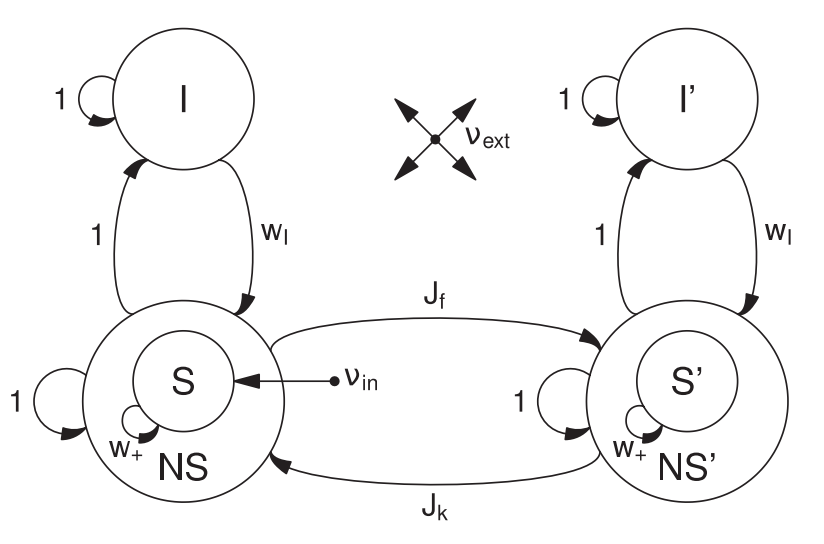
\includegraphics[scale = 0.75]{Buehlmann2010_Schema}
\caption{Schematic representation of the network used by Buehlmann and Deco. ``The network consists of two parts. In each part, there are excitatory (S, NS) and inhibitory (I) neurons.'' \cite{Buehlmann2010}}
\label{Buehlmann2010_Schema}
\end{figure}

The second model will follow that used by Bhowmik and Shanahan and is depicted in Figure \ref{Bhowmik2013_Schema}.

\begin{figure}[H]
\centering
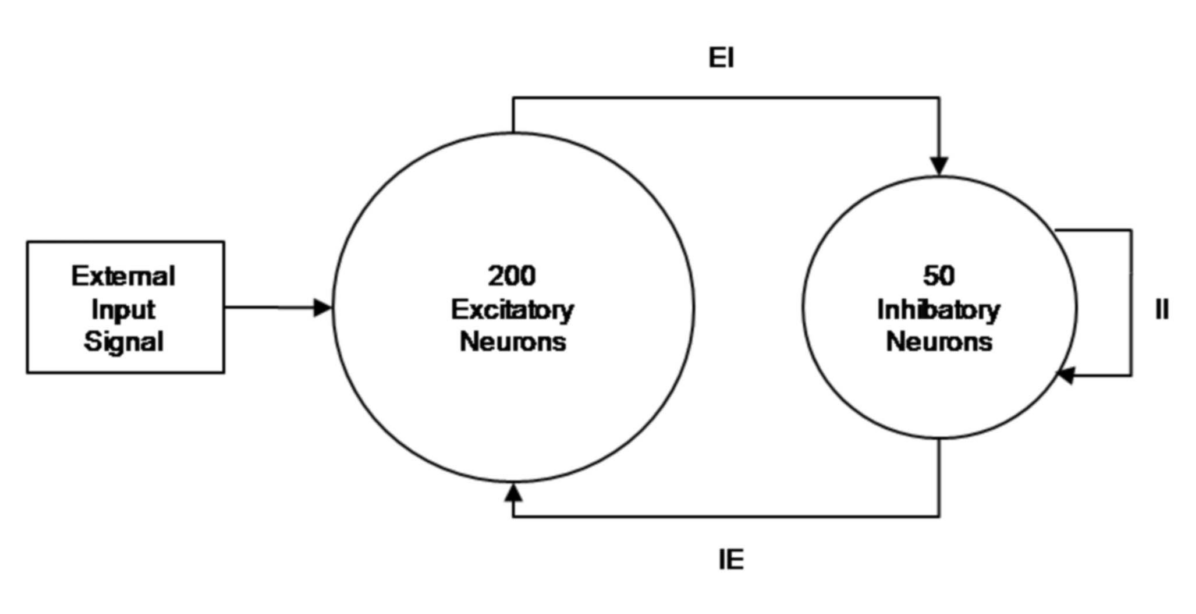
\includegraphics[scale = 0.75]{Bhowmik2013_Schema}
\caption{``The pyramidal inter-neuronal gamma (PING) architecture used for the neural oscillator nodes in the simulation experiments. To generate oscillator nodes of different frequencies for different neural models this base architecture was used with a genetic algorithm evolving the weights and delays for the synaptic connections.'' \cite{Bhowmik2013}}
\label{Bhowmik2013_Schema}
\end{figure}

\subsection{Analysis}

Having run a number of simulations as described in \ref{MSUKO} and \ref{MSUSNN}, the output generated by these will be used to calculated the network's integrated information. We will then run an analysis to investigate whether there are any connections between the properties of each network and its integrated information.

\subsection{Ensure Robustness of $\Phi$ Implementation for JIDT}

One of the objectives of this project is to make the implementation of $\Phi$ for JIDT robust enough that it is included in the official distribution. In order to do this, once an initial working version of the implementation is finalised, we will send it to Lizier, who maintains the toolkit. By collaborating with Lizier, we aim to make conducting studies into integrated information using time series data more easily accessible for other researchers.

\subsubsection{Other Versions of $\Phi$}
Currently we have a working implementation of $\Phi_{E}$. In order to provide the user with flexibility, we aim to extend our contribution to JIDT to include other versions of $\Phi$ such as $\Phi_{DM}$ and $\Phi_{AR}$. This will allow the user to easily test the discrepancies between the different measures.

\subsubsection{Smoothing using Dirichlet Distribution}
The JIDT currently calculates mutual information for discrete data without taking into account the possibility that a state has not been observed given a relatively small input. This causes the probability of those unobserved states to be zero, potentially giving a skewed picture of the probability distribution. In order to correct for this, we will overload the JIDT's mutual information calculator for discrete data so that it can take an extra parameter $\alpha$. With this term we can then smooth the posterior distribution of the input data using a symmetric Dirichlet distribution with $\alpha$ as a prior.

\subsubsection{Testing}
In order to ensure that our implementation follows good software engineering practices and aligns itself with the tests provided by JIDT, we will write a variety of tests to cover both common and edge cases of our implementations of $\Phi$ and $\phi$ as well as our helper classes. We will do this using JUnit, as this is the testing framework used by default by JIDT.


% ==========
% References
% ==========
\clearpage
\bibliography{report}{}
\bibliographystyle{plain}
\clearpage

\end{document}